\documentclass[11pt,a4paper]{article}

% ---------- Codificación e idioma ----------
\usepackage[utf8]{inputenc}
\usepackage[T1]{fontenc}
\usepackage{lmodern}
\usepackage[spanish]{babel}

% ---------- Matemáticas, figuras y tablas ----------
\usepackage{amsmath}
\usepackage{amssymb}
\usepackage{graphicx}
\usepackage{booktabs}
\usepackage{float}
\usepackage{caption}
\usepackage{geometry}
\geometry{margin=2.5cm}
\usepackage{xcolor}
\usepackage{listings}
\usepackage[hidelinks]{hyperref}

\captionsetup{font=small,labelfont=bf}
\setlength{\parindent}{0pt}
\setlength{\parskip}{0.6em}


% ---------- Estilo de los fragmentos de código ----------
\lstset{
    language=Python,
    basicstyle=\ttfamily\small,
    keywordstyle=\color{blue!60!black}\bfseries,
    commentstyle=\color{green!40!black}\itshape,
    stringstyle=\color{red!60!black},
    backgroundcolor=\color{gray!6},
    frame=single,
    rulecolor=\color{gray!40},
    breaklines=true,
    columns=fullflexible,
    keepspaces=true,
    showstringspaces=false,
    numbers=left,
    numberstyle=\tiny\color{gray},
    xleftmargin=1.5em,
    framexleftmargin=1.5em,
    literate={á}{{\'a}}1 {é}{{\'e}}1 {í}{{\'i}}1 {ó}{{\'o}}1 {ú}{{\'u}}1
             {Á}{{\'A}}1 {É}{{\'E}}1 {Í}{{\'I}}1 {Ó}{{\'O}}1 {Ú}{{\'U}}1
             {ñ}{{\~n}}1 {Ñ}{{\~N}}1 {¿}{{?`}}1 {¡}{{!`}}1
}

\newcommand{\dd}{\mathrm{d}}
\newcommand{\E}{\mathbb{E}}
\newcommand{\Var}{\operatorname{Var}}
\newcommand{\Med}{\operatorname{Med}}

\title{\textbf{Movimiento browniano geométrico:\\solución exacta, Euler-Maruyama y simulación con \texttt{diffeqpy}}}
\author{Curso de Modelación Matemática}
\date{\today}

\begin{document}
\maketitle

\begin{abstract}
\noindent
Se estudia la ecuación diferencial estocástica del movimiento browniano geométrico (MBG), $\dd X_t = \mu X_t\,\dd t + \sigma X_t\,\dd B_t$, comparándola con su modelo determinista $\dot x = \mu x$. A partir del lema de Itô se obtiene la solución exacta, su media $X_0e^{\mu t}$, su mediana $X_0e^{(\mu-\sigma^2/2)t}$ y su varianza, y se demuestra que $P(X_T < x(T)) = \Phi(\sigma\sqrt{T}/2)$. Las trayectorias se simulan con el esquema de Euler-Maruyama de la biblioteca \texttt{DifferentialEquations.jl}, usada desde Python mediante \texttt{diffeqpy}. Con $X_0 = 0$ la simulación coincide exactamente con la solución determinista (diferencia máxima $0$). Con los parámetros de la clase ($\mu = 0.25$, $\sigma = 1$, $X_0 = 1$, $T = 10$) la media teórica en $t = T$ es $12.1825$, pero la mediana es $0.0821$: la media muestral de 20 trayectorias fue $0.8444$ y, de 10 trayectorias, las 10 terminaron por debajo del modelo determinista (probabilidad teórica 94.3\,\%). Se explica por qué la media crece mientras casi todas las trayectorias decaen, y qué cambia cuando $\sigma^2 < 2\mu$.
\end{abstract}

\tableofcontents
\newpage

% ============================================================
\section{Introducción}
% ============================================================

Muchos fenómenos crecen de forma proporcional a su tamaño: una población, un capital invertido o la concentración de un reactivo autocatalítico. El modelo más simple es la ecuación diferencial ordinaria $\dot x = \mu x$, cuya solución es la exponencial $x(t) = X_0 e^{\mu t}$. Cuando la tasa de crecimiento no es constante sino que fluctúa de manera aleatoria, el modelo se convierte en una ecuación diferencial estocástica (EDE): el \emph{movimiento browniano geométrico}.

El objetivo de este trabajo es:
\begin{enumerate}
    \item deducir la solución exacta del MBG con el lema de Itô y sus momentos (media, mediana y varianza);
    \item deducir y explicar el esquema numérico de Euler-Maruyama y sus órdenes de convergencia;
    \item describir cómo se usa la biblioteca \texttt{diffeqpy} para resolver la EDE y la EDO desde Python;
    \item explicar el código de los tres scripts del proyecto:
    \begin{itemize}
        \item \texttt{simulacion\_mbg.py},
        \item \texttt{simulacion\_mbg\_clase.py},
        \item \texttt{simulacion\_mbg\_vs\_determinista.py};
    \end{itemize}
    \item comparar los resultados simulados con la teoría e interpretar por qué la media del proceso crece mientras la mayoría de las trayectorias decae.
\end{enumerate}

% ============================================================
\section{Modelo}
% ============================================================

\subsection{La ecuación diferencial estocástica}

El MBG es la solución de
\begin{equation}
    \dd X_t = \underbrace{\mu X_t\,\dd t}_{\text{deriva}} \;+\; \underbrace{\sigma X_t\,\dd B_t}_{\text{difusión}},
    \qquad X_0 \text{ dado},
    \label{eq:ede}
\end{equation}
donde $\mu$ es la \emph{deriva} (tasa media de crecimiento), $\sigma > 0$ la \emph{volatilidad} y $B_t$ un movimiento browniano estándar: $B_0 = 0$, incrementos independientes y $B_t - B_s \sim N(0,\,t-s)$.

\begin{itemize}
    \item \textbf{Parte determinista.} Si $\sigma = 0$, la ecuación~\eqref{eq:ede} se reduce a la EDO
    \begin{equation}
        \frac{\dd x}{\dd t} = \mu x \quad\Longrightarrow\quad x(t) = X_0 e^{\mu t}.
        \label{eq:edo}
    \end{equation}
    En este informe $x(t)$ se llama \emph{modelo determinista}.
    \item \textbf{Parte con ruido.} El término $\sigma X_t\,\dd B_t$ añade perturbaciones aleatorias. Formalmente, \eqref{eq:ede} equivale a $\dot X = (\mu + \sigma \xi_t) X$, con $\xi_t$ ruido blanco: la tasa de crecimiento fluctúa alrededor de $\mu$.
    \item \textbf{Ruido multiplicativo.} La intensidad del ruido es proporcional al estado, $g(X) = \sigma X$. Dos consecuencias: (i) las fluctuaciones relativas $\dd X/X$ tienen siempre el mismo tamaño, y (ii) si $X_0 = 0$ ambos términos se anulan y $X_t \equiv 0$ es solución: el ruido no puede sacar al proceso del cero. Lo mismo vale para el esquema numérico (sección~\ref{sec:em}).
\end{itemize}

\subsection{Solución exacta por el lema de Itô}

\textbf{Lema de Itô (una dimensión).} Si $\dd X_t = a(X_t)\,\dd t + b(X_t)\,\dd B_t$ y $F$ es dos veces derivable, entonces
\begin{equation}
    \dd F(X_t) = \left( F'(X_t)\,a + \tfrac12 F''(X_t)\,b^2 \right)\dd t + F'(X_t)\,b\,\dd B_t .
    \label{eq:ito}
\end{equation}
El término $\tfrac12 F'' b^2$ no aparece en el cálculo ordinario; proviene de que $(\dd B_t)^2 = \dd t$: el incremento browniano es de tamaño $\sqrt{\dd t}$, por lo que su cuadrado es del mismo orden que $\dd t$ y no se puede despreciar.

Con $F(X) = \ln X$, $F' = 1/X$, $F'' = -1/X^2$, $a = \mu X$ y $b = \sigma X$:
\begin{equation}
    \dd(\ln X_t) = \left( \mu - \frac{\sigma^2}{2} \right)\dd t + \sigma\,\dd B_t .
\end{equation}
El lado derecho ya no depende de $X_t$, así que se integra directamente entre $0$ y $t$:
\begin{equation}
    \boxed{X_t = X_0 \exp\!\left[ \left( \mu - \frac{\sigma^2}{2} \right) t + \sigma B_t \right]}
    \label{eq:solucion}
\end{equation}
Por tanto $\ln X_t \sim N\!\big(\ln X_0 + (\mu - \sigma^2/2)t,\ \sigma^2 t\big)$: $X_t$ tiene distribución lognormal (para $X_0 > 0$).

\subsection{Media, mediana y varianza}

Si $Z \sim N(m, s^2)$, entonces $\E[e^Z] = e^{m + s^2/2}$ y $\E[e^{2Z}] = e^{2m + 2s^2}$. Con $m = \ln X_0 + (\mu - \sigma^2/2)t$ y $s^2 = \sigma^2 t$:
\begin{align}
    \E[X_t]   &= X_0 e^{\mu t}, \label{eq:media}\\
    \Med[X_t] &= X_0 e^{(\mu - \sigma^2/2)t}, \label{eq:mediana}\\
    \Var[X_t] &= X_0^2 e^{2\mu t}\left( e^{\sigma^2 t} - 1 \right). \label{eq:varianza}
\end{align}
La mediana se obtiene porque $e^{Z}$ es creciente: la mediana de $e^Z$ es $e^{\text{mediana de }Z} = e^m$.

\textbf{La media del MBG es exactamente el modelo determinista}~\eqref{eq:edo}. Esto se ve también tomando esperanza en~\eqref{eq:ede}: como $\E\!\left[\int_0^t \sigma X_s\,\dd B_s\right] = 0$ (propiedad de la integral de Itô), $m(t) = \E[X_t]$ cumple $\dot m = \mu m$.

\subsection{\texorpdfstring{La corrección $-\sigma^2/2$}{La corrección -sigma²/2}}

La tasa de crecimiento \emph{típica} de una trayectoria no es $\mu$ sino
\begin{equation}
    \lambda = \mu - \frac{\sigma^2}{2},
    \qquad \lim_{t\to\infty} \frac{\ln X_t}{t} = \lambda \quad \text{casi seguramente},
\end{equation}
porque $B_t/t \to 0$ (ley fuerte de los grandes números para el browniano). En consecuencia:
\begin{itemize}
    \item si $\sigma^2 < 2\mu$ ($\lambda > 0$), casi todas las trayectorias crecen;
    \item si $\sigma^2 > 2\mu$ ($\lambda < 0$), casi todas las trayectorias tienden a cero, \emph{aunque la media $X_0e^{\mu t}$ crezca sin límite}.
\end{itemize}
La explicación intuitiva: una ganancia del $+50$\,\% seguida de una pérdida del $-50$\,\% deja el valor en $1.5 \times 0.5 = 0.75$; las fluctuaciones multiplicativas simétricas reducen el crecimiento compuesto. La cantidad que se pierde es justamente $\sigma^2/2$ por unidad de tiempo.

\subsection{Probabilidad de terminar por debajo del modelo determinista}

Usando~\eqref{eq:solucion} y $x(T) = X_0e^{\mu T}$ (con $X_0 > 0$):
\begin{align}
    P\big(X_T < x(T)\big)
    &= P\!\left( \left(\mu - \tfrac{\sigma^2}{2}\right)T + \sigma B_T < \mu T \right)
     = P\!\left( B_T < \tfrac{\sigma T}{2} \right) \nonumber\\
    &= P\!\left( \frac{B_T}{\sqrt{T}} < \frac{\sigma\sqrt{T}}{2} \right)
     = \boxed{\Phi\!\left( \frac{\sigma\sqrt{T}}{2} \right)}
    \label{eq:prob}
\end{align}
donde $\Phi$ es la función de distribución normal estándar. El resultado no depende de $\mu$ ni de $X_0$ y es siempre mayor que $1/2$: \textbf{la mayoría de las trayectorias termina por debajo de la media}. Para $\sigma = 1$ y $T = 10$, $\Phi(1.581) = 0.943$.

% ============================================================
\section{Método numérico: Euler-Maruyama}
\label{sec:em}
% ============================================================

\subsection{Deducción del esquema}

La EDE~\eqref{eq:ede} significa, por definición, la ecuación integral
\begin{equation}
    X_{t_{n+1}} = X_{t_n} + \int_{t_n}^{t_{n+1}} \mu X_s\,\dd s + \int_{t_n}^{t_{n+1}} \sigma X_s\,\dd B_s .
\end{equation}
Se divide $[0,T]$ en $N$ pasos de tamaño $\Delta t = T/N$, $t_n = n\Delta t$. Si en cada subintervalo se \emph{congela} el integrando en su valor del extremo izquierdo, $X_s \approx X_{t_n}$ (lo mismo que hace el método de Euler explícito para EDO, y coherente con la definición de la integral de Itô, que evalúa en el extremo izquierdo), se obtiene
\begin{equation}
    \boxed{X_{n+1} = X_n + \mu X_n\,\Delta t + \sigma X_n\,\Delta B_n,
    \qquad \Delta B_n = B_{t_{n+1}} - B_{t_n}}
    \label{eq:em}
\end{equation}
Con $\sigma = 0$ el esquema se reduce al método de Euler para $\dot x = \mu x$.

\subsection{El incremento browniano}

Por la definición del movimiento browniano,
\begin{equation}
    \Delta B_n \sim N(0, \Delta t)
    \quad\Longrightarrow\quad
    \Delta B_n = \sqrt{\Delta t}\; Z_n, \qquad Z_n \sim N(0,1) \text{ independientes}.
\end{equation}
En cada paso basta con generar un número normal estándar y multiplicarlo por $\sqrt{\Delta t}$ (no por $\Delta t$). Observe que el término aleatorio es de orden $\sqrt{\Delta t}$, mucho mayor que el término de deriva, de orden $\Delta t$, cuando $\Delta t$ es pequeño. La semilla del generador fija la sucesión $Z_n$ y hace la trayectoria reproducible.

Como $X_{n+1} = X_n\,(1 + \mu\Delta t + \sigma\Delta B_n)$, si $X_0 = 0$ todos los $X_n$ son exactamente cero, sin importar el valor de los $\Delta B_n$.

\subsection{Órdenes de convergencia}

Sea $X_N$ la aproximación numérica en $t = T$ y $X(T)$ la solución exacta obtenida \emph{con el mismo camino browniano}.

\begin{itemize}
    \item \textbf{Convergencia fuerte (camino a camino), orden $1/2$:}
    \begin{equation}
        \E\,|X_N - X(T)| \le C\,\Delta t^{1/2}.
    \end{equation}
    Mide qué tan cerca está cada trayectoria simulada de la verdadera. Reducir el error a la mitad exige un $\Delta t$ cuatro veces menor. La pérdida de orden respecto a Euler para EDO (orden 1) se debe a que el esquema ignora el término $\tfrac12\sigma^2 X\big((\Delta B)^2 - \Delta t\big)$ del desarrollo de Itô-Taylor, que tiene tamaño $\Delta t$ por paso pero no se cancela en media cuadrática; el método de Milstein lo incluye y alcanza orden fuerte 1.
    \item \textbf{Convergencia débil (en distribución), orden $1$:}
    \begin{equation}
        \big|\E[\varphi(X_N)] - \E[\varphi(X(T))]\big| \le C\,\Delta t
    \end{equation}
    para funciones $\varphi$ suaves. Mide qué tan bien se aproximan la media, la varianza y otras estadísticas. Por ejemplo, tomando esperanza en~\eqref{eq:em}, $\E[X_N] = X_0(1 + \mu\Delta t)^N$, que converge a $X_0e^{\mu T}$ con error $O(\Delta t)$.
\end{itemize}

\subsection{\texorpdfstring{Por qué importa $\Delta t$}{Por qué importa dt}}

\begin{itemize}
    \item El error de cada trayectoria decrece solo como $\sqrt{\Delta t}$; con $\Delta t$ grande las trayectorias se deforman.
    \item El factor $1 + \mu\Delta t + \sigma\sqrt{\Delta t}\,Z_n$ puede ser negativo si $\sigma\sqrt{\Delta t}$ no es pequeño, mientras que la solución exacta~\eqref{eq:solucion} es siempre positiva. Con $\sigma = 1$ y $\Delta t = 0.01$ se necesitaría $Z_n < -10.025$, algo prácticamente imposible; con $\Delta t = 0.25$ bastaría $Z_n < -2.125$ (aproximadamente un 1.7\,\% de los pasos).
    \item Hay que distinguir dos fuentes de error: el error de discretización, controlado por $\Delta t$, y el error de muestreo (Monte Carlo), controlado por el número de trayectorias $M$. En este problema el segundo domina, como se verá en la sección~\ref{sec:discusion}.
\end{itemize}

% ============================================================
\section{La biblioteca \texttt{diffeqpy}}
% ============================================================

\subsection{Qué es}

\texttt{diffeqpy} es la interfaz de Python para \texttt{DifferentialEquations.jl}, el ecosistema de resolución de ecuaciones diferenciales del lenguaje Julia (proyecto SciML). Desde Python se definen las funciones del modelo y se llama a los mismos objetos y algoritmos de Julia (\texttt{ODEProblem}, \texttt{SDEProblem}, \texttt{solve}, \texttt{Tsit5}, \texttt{EM}, \ldots). La comunicación entre los dos lenguajes la hace \texttt{juliacall} (paquete PythonCall/JuliaCall).

\subsection{Instalación}

\begin{enumerate}
    \item \textbf{Julia con juliaup}, el instalador oficial de versiones de Julia (queda en \verb|~/.juliaup/bin|):
\begin{verbatim}
curl -fsSL https://install.julialang.org | sh
export PATH="$HOME/.juliaup/bin:$PATH"
\end{verbatim}
    \item \textbf{Paquetes de Python} en el entorno virtual \texttt{venv/} (instala \texttt{juliacall} como dependencia):
\begin{verbatim}
source venv/bin/activate
pip install diffeqpy numpy matplotlib
\end{verbatim}
    \item \textbf{Paquetes de Julia} (\texttt{DifferentialEquations.jl} y sus dependencias), una sola vez:
\begin{verbatim}
python3 -c "from diffeqpy import install; install()"
\end{verbatim}
\end{enumerate}
Versiones usadas en este informe: Python 3.14.4, Julia 1.13.3, \texttt{diffeqpy} 2.6.0 y \texttt{juliacall} 0.9.37. La primera instrucción \texttt{from diffeqpy import de} de cada sesión tarda porque Julia compila los métodos; no es un cuelgue. Julia debe estar en el \texttt{PATH}.

\subsection{Cómo se usa en el código}

\begin{table}[H]
    \centering
    \caption{Elementos de \texttt{diffeqpy} que aparecen en los scripts.}
    \label{tab:diffeqpy}
    \begin{tabular}{p{4.2cm}p{10.3cm}}
        \toprule
        Elemento & Función en el código \\
        \midrule
        \texttt{f(u, p, t)}, \texttt{g(u, p, t)} & Deriva $\mu u$ y difusión $\sigma u$. Reciben el estado \texttt{u}, los parámetros \texttt{p = (mu, sigma)} y el tiempo \texttt{t}. \\
        \texttt{de.ODEProblem(f, X0, (0, T), p)} & Define la EDO $\dot x = f(x)$, es decir, el modelo determinista. \\
        \texttt{de.SDEProblem(f, g, X0, (0, T), p)} & Define la EDE $\dd X = f\,\dd t + g\,\dd B$ (ruido diagonal de Itô). \\
        \texttt{de.Tsit5()} & Runge-Kutta explícito de Tsitouras de orden 5(4) con paso adaptativo; resuelve la EDO con error muy pequeño. \\
        \texttt{de.EM()} & Euler-Maruyama, ec.~\eqref{eq:em}. Es de paso fijo, por eso exige \texttt{dt}. \\
        \texttt{dt} & Tamaño del paso $\Delta t$ de Euler-Maruyama. \\
        \texttt{saveat=dt} & Instantes en que se guarda la solución: la malla $0, \Delta t, \ldots, T$. En \texttt{Tsit5} los valores se obtienen por interpolación, así la EDO y la EDE quedan en la misma malla. \\
        \texttt{seed=k} & Semilla del generador de los $\Delta B_n$: cada $k$ da una trayectoria distinta pero reproducible. \\
        \texttt{sol.t}, \texttt{sol.u} & Tiempos y valores de la solución; se convierten a arreglos con \texttt{np.array}. \\
        \bottomrule
    \end{tabular}
\end{table}

% ============================================================
\section{Explicación del código}
% ============================================================

Los tres scripts comparten la misma estructura: (1) leer parámetros, (2) definir $f$ y $g$, (3) resolver la EDO y/o la EDE con \texttt{diffeqpy}, (4) imprimir estadísticas y (5) guardar una figura PNG.

\subsection{\texorpdfstring{Núcleo común: coeficientes y $M$ trayectorias}{Núcleo común: coeficientes y M trayectorias}}

\begin{lstlisting}
def f(u, p, t):          # deriva (parte determinista)
    return p[0] * u

def g(u, p, t):          # difusión (parte estocástica)
    return p[1] * u

prob = de.SDEProblem(f, g, X0, (0.0, T), (mu, sigma))
X = np.array([np.array(de.solve(prob, de.EM(), dt=dt, saveat=dt, seed=args.seed + k).u)
              for k in range(M)])                 # forma (M, n_pasos)
\end{lstlisting}

El problema se define una sola vez y se resuelve $M$ veces cambiando la semilla (\texttt{seed + k}). Cada solución es un vector de $N + 1 = T/\Delta t + 1$ valores; al apilarlos se obtiene una matriz de forma $(M, N+1)$, donde la fila $k$ es la trayectoria $k$ y la columna $n$ es el instante $t_n$. Así, \texttt{X.mean(axis=0)} es la media muestral en cada instante y \texttt{X[:, -1]} contiene los valores finales $X_T$.

\subsection{\texorpdfstring{\texttt{simulacion\_mbg.py}: el caso $X_0 = 0$}{simulacion\_mbg.py: el caso X0 = 0}}

Es la primera versión del estudio. Los parámetros están escritos en el código (versión del último commit):

\begin{lstlisting}
mu, sigma = 0.5, 0.3     # deriva y volatilidad
X0 = 0.0                 # condición inicial
T, dt = 1.0, 0.01        # horizonte y paso de tiempo
M = 20                   # número de trayectorias
p = [mu, sigma]

prob_ode = de.ODEProblem(f, X0, (0.0, T), p)
sol_ode = de.solve(prob_ode, de.Tsit5(), saveat=dt)
x_exacta = X0 * np.exp(mu * t)
...
dif = np.abs(X - x_det)
\end{lstlisting}

Resuelve la EDO con \texttt{Tsit5}, la compara con la solución analítica $X_0e^{\mu t}$ (verificación del integrador), simula 20 trayectorias con \texttt{EM} (semillas $1,\ldots,20$) y calcula la diferencia máxima $\max_k |X_t^{(k)} - x(t)|$ en cada instante. La figura tiene dos paneles: trayectorias, promedio y modelo determinista; y la diferencia máxima en función del tiempo.

Nota: al ejecutarlo, Julia emite un aviso de rendimiento porque \texttt{p} es una lista de Python; \texttt{DifferentialEquations.jl} recomienda pasar los parámetros como tupla, como hacen los otros dos scripts. No afecta los resultados.

\subsection{\texttt{simulacion\_mbg\_clase.py}: el caso de la clase}

Es la versión principal. Lee los parámetros desde la terminal con \texttt{argparse}, de modo que no hay que editar el código para cambiar $\mu$, $\sigma$, $X_0$, $T$, $\Delta t$, $M$ o la semilla:

\begin{lstlisting}
parser.add_argument("--mu", type=float, default=0.25, help="deriva (default 0.25)")
parser.add_argument("--sigma", type=float, default=1.0, help="volatilidad (default 1.0)")
...
args = parser.parse_args()
from diffeqpy import de   # se importa después de leer los argumentos
\end{lstlisting}

La importación de \texttt{diffeqpy} va después de \texttt{parse\_args()} para que \texttt{--help} responda de inmediato, sin esperar a que arranque Julia. Después de simular, compara las trayectorias con las curvas teóricas~\eqref{eq:media} y~\eqref{eq:mediana}:

\begin{lstlisting}
media = X0 * np.exp(mu * t)
mediana = X0 * np.exp((mu - sigma**2 / 2) * t)
print(f"t = T:  media muestral = {X[:, -1].mean():.4f}   mediana muestral = {np.median(X[:, -1]):.4f}")
\end{lstlisting}

La figura usa eje $y$ logarítmico por defecto (opción \texttt{--lineal} para cambiarlo). En escala logarítmica, $\ln X_t$ es un browniano con deriva $\lambda$, así que la mediana es una recta y las trayectorias se distribuyen de forma simétrica alrededor de ella.

\subsection{\texttt{simulacion\_mbg\_vs\_determinista.py}: trayectorias frente al modelo determinista}

Tiene las mismas opciones de línea de comandos (sin \texttt{--lineal}). Resuelve el modelo determinista con \texttt{Tsit5} y las $M$ trayectorias con \texttt{EM}, y cuenta cuántas terminan por debajo de $x(T)$, comparando con la probabilidad teórica~\eqref{eq:prob}:

\begin{lstlisting}
abajo = int(np.sum(X[:, -1] < x_det[-1]))
p_teo = 0.5 * (1 + erf((sigma * sqrt(T) / 2) / sqrt(2)))   # Phi(sigma sqrt(T) / 2)
\end{lstlisting}

La función $\Phi$ se calcula con la función error, $\Phi(z) = \tfrac12\big[1 + \operatorname{erf}(z/\sqrt2)\big]$, sin necesidad de \texttt{scipy}. La figura muestra las mismas curvas en escala lineal (izquierda) y logarítmica (derecha, con la mediana teórica).

% ============================================================
\section{Resultados}
% ============================================================

Los scripts se ejecutaron sin ventana gráfica (\texttt{MPLBACKEND=Agg}); las figuras se guardaron en \texttt{figuras\_informe\_mbg/}. Todos los números de esta sección son los que imprimieron esas ejecuciones.

\subsection{\texorpdfstring{Caso $X_0 = 0$: solución trivial}{Caso X0 = 0: solución trivial}}

Parámetros: $\mu = 0.5$, $\sigma = 0.3$, $X_0 = 0$, $T = 1$, $\Delta t = 0.01$, $M = 20$.

\begin{table}[H]
    \centering
    \caption{Salida de \texttt{simulacion\_mbg.py} con $X_0 = 0$.}
    \label{tab:x0}
    \begin{tabular}{lr}
        \toprule
        Cantidad & Valor \\
        \midrule
        $\max_t |x_{\text{Tsit5}}(t) - X_0e^{\mu t}|$ & $0.000\times10^{0}$ \\
        $\max_{k,t} |X^{(k)}_t - x(t)|$ (Euler-Maruyama $-$ determinista) & $0.000\times10^{0}$ \\
        Promedio EM en $t = T$ & 0.0000 \\
        Determinista $x(T)$ & 0.0000 \\
        \bottomrule
    \end{tabular}
\end{table}

\begin{figure}[H]
    \centering
    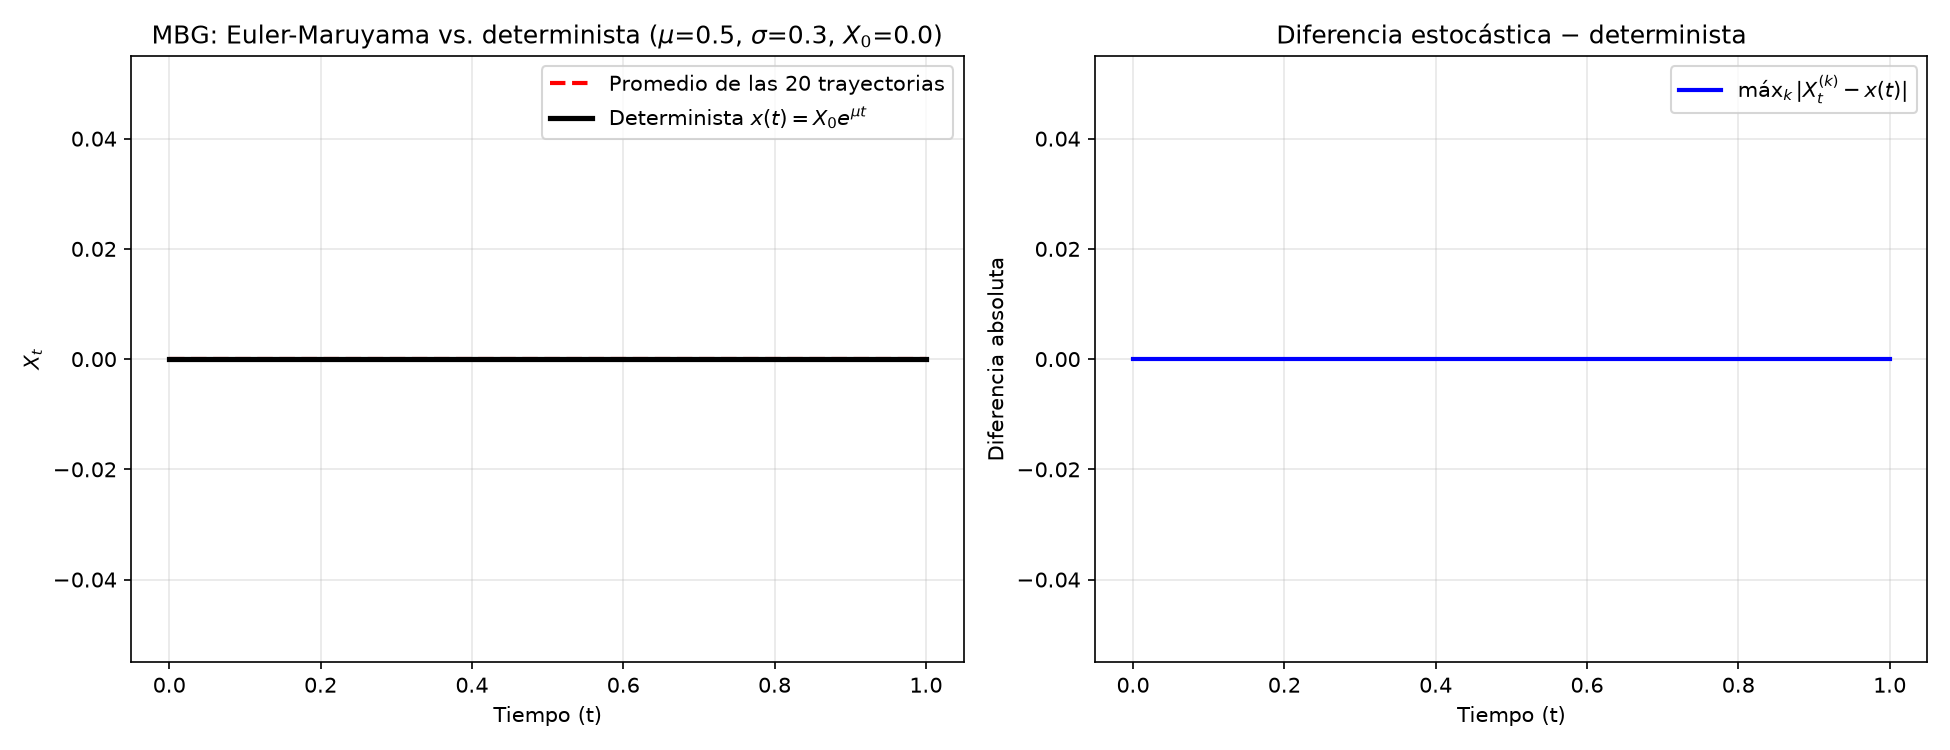
\includegraphics[width=\linewidth]{figuras_informe_mbg/resultado_mbg.png}
    \caption{Caso $X_0 = 0$. Izquierda: las 20 trayectorias de Euler-Maruyama, su promedio y el modelo determinista coinciden con la recta $X \equiv 0$. Derecha: la diferencia máxima entre las trayectorias y el modelo determinista es cero en todo instante.}
    \label{fig:x0}
\end{figure}

Las diferencias son exactamente cero, no solo pequeñas, porque con ruido multiplicativo cada paso es $X_{n+1} = X_n(1 + \mu\Delta t + \sigma\Delta B_n) = 0$. Este caso sirve como prueba de consistencia del código: confirma que el ruido entra multiplicado por el estado.

\subsection{\texorpdfstring{Caso de la clase: $\mu = 0.25$, $\sigma = 1$, $X_0 = 1$, $T = 10$, 20 trayectorias}{Caso de la clase: mu = 0.25, sigma = 1, X0 = 1, T = 10, 20 trayectorias}}

Parámetros: $\Delta t = 0.01$ (1000 pasos), semillas $1,\ldots,20$. Como $\lambda = \mu - \sigma^2/2 = -0.25 < 0$, la mediana decrece.

\begin{table}[H]
    \centering
    \caption{Salida de \texttt{simulacion\_mbg\_clase.py} con los parámetros por defecto, en $t = T = 10$.}
    \label{tab:clase}
    \begin{tabular}{lrr}
        \toprule
        Estadístico & Teórico & Muestral ($M = 20$) \\
        \midrule
        $\mu - \sigma^2/2$ & $-0.2500$ & --- \\
        Media $\E[X_T]$     & 12.1825 & 0.8444 \\
        Mediana $\Med[X_T]$ & 0.0821  & 0.0515 \\
        \bottomrule
    \end{tabular}
\end{table}

\begin{figure}[H]
    \centering
    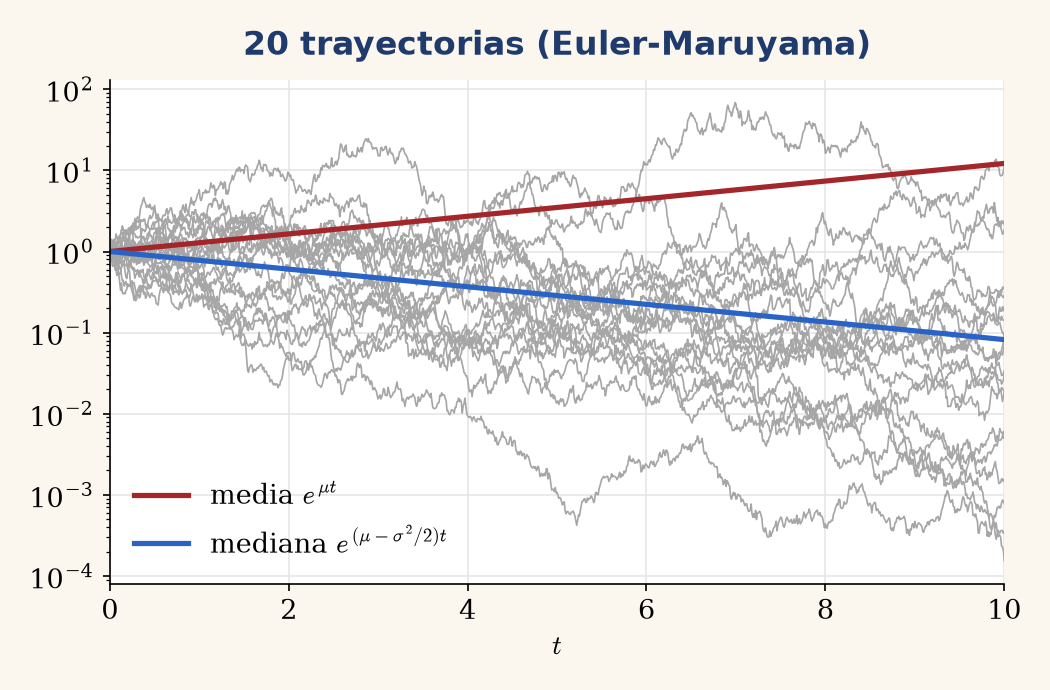
\includegraphics[width=0.85\linewidth]{figuras_informe_mbg/resultado_mbg_clase.png}
    \caption{Veinte trayectorias de Euler-Maruyama (gris) con $\mu = 0.25$, $\sigma = 1$, $X_0 = 1$, en escala logarítmica. La media teórica $e^{\mu t}$ (rojo) crece, mientras que la mediana $e^{(\mu - \sigma^2/2)t}$ (azul) decrece; las trayectorias se agrupan alrededor de la mediana.}
    \label{fig:clase}
\end{figure}

La mediana muestral ($0.0515$) es del mismo orden que la teórica ($0.0821$), mientras que la media muestral ($0.8444$) es unas 14 veces menor que la teórica ($12.1825$).

\subsection{Diez trayectorias frente al modelo determinista}

Mismos parámetros que el caso anterior, con $M = 10$ (semillas $1,\ldots,10$).

\begin{table}[H]
    \centering
    \caption{Resumen de \texttt{simulacion\_mbg\_vs\_determinista.py} con $M = 10$, en $t = T = 10$.}
    \label{tab:vsdet}
    \begin{tabular}{lr}
        \toprule
        Cantidad & Valor \\
        \midrule
        Modelo determinista $x(T)$          & 12.1825 \\
        Promedio de las 10 trayectorias     & 1.3498 \\
        Mediana teórica                     & 0.0821 \\
        Trayectorias por debajo de $x(T)$   & 10 de 10 (100\,\%) \\
        Probabilidad teórica $\Phi(\sigma\sqrt{T}/2)$ & 94.3\,\% \\
        \bottomrule
    \end{tabular}
\end{table}

\begin{table}[H]
    \centering
    \caption{Valor final de cada trayectoria.}
    \label{tab:finales}
    \begin{tabular}{crl}
        \toprule
        Trayectoria & $X_T$ & Posición respecto a $x(T) = 12.1825$ \\
        \midrule
        1  & 1.8517  & debajo \\
        2  & 0.1434  & debajo \\
        3  & 11.3090 & debajo \\
        4  & 0.0317  & debajo \\
        5  & 0.0184  & debajo \\
        6  & 0.0862  & debajo \\
        7  & 0.0182  & debajo \\
        8  & 0.0052  & debajo \\
        9  & 0.0002  & debajo \\
        10 & 0.0339  & debajo \\
        \bottomrule
    \end{tabular}
\end{table}

\begin{figure}[H]
    \centering
    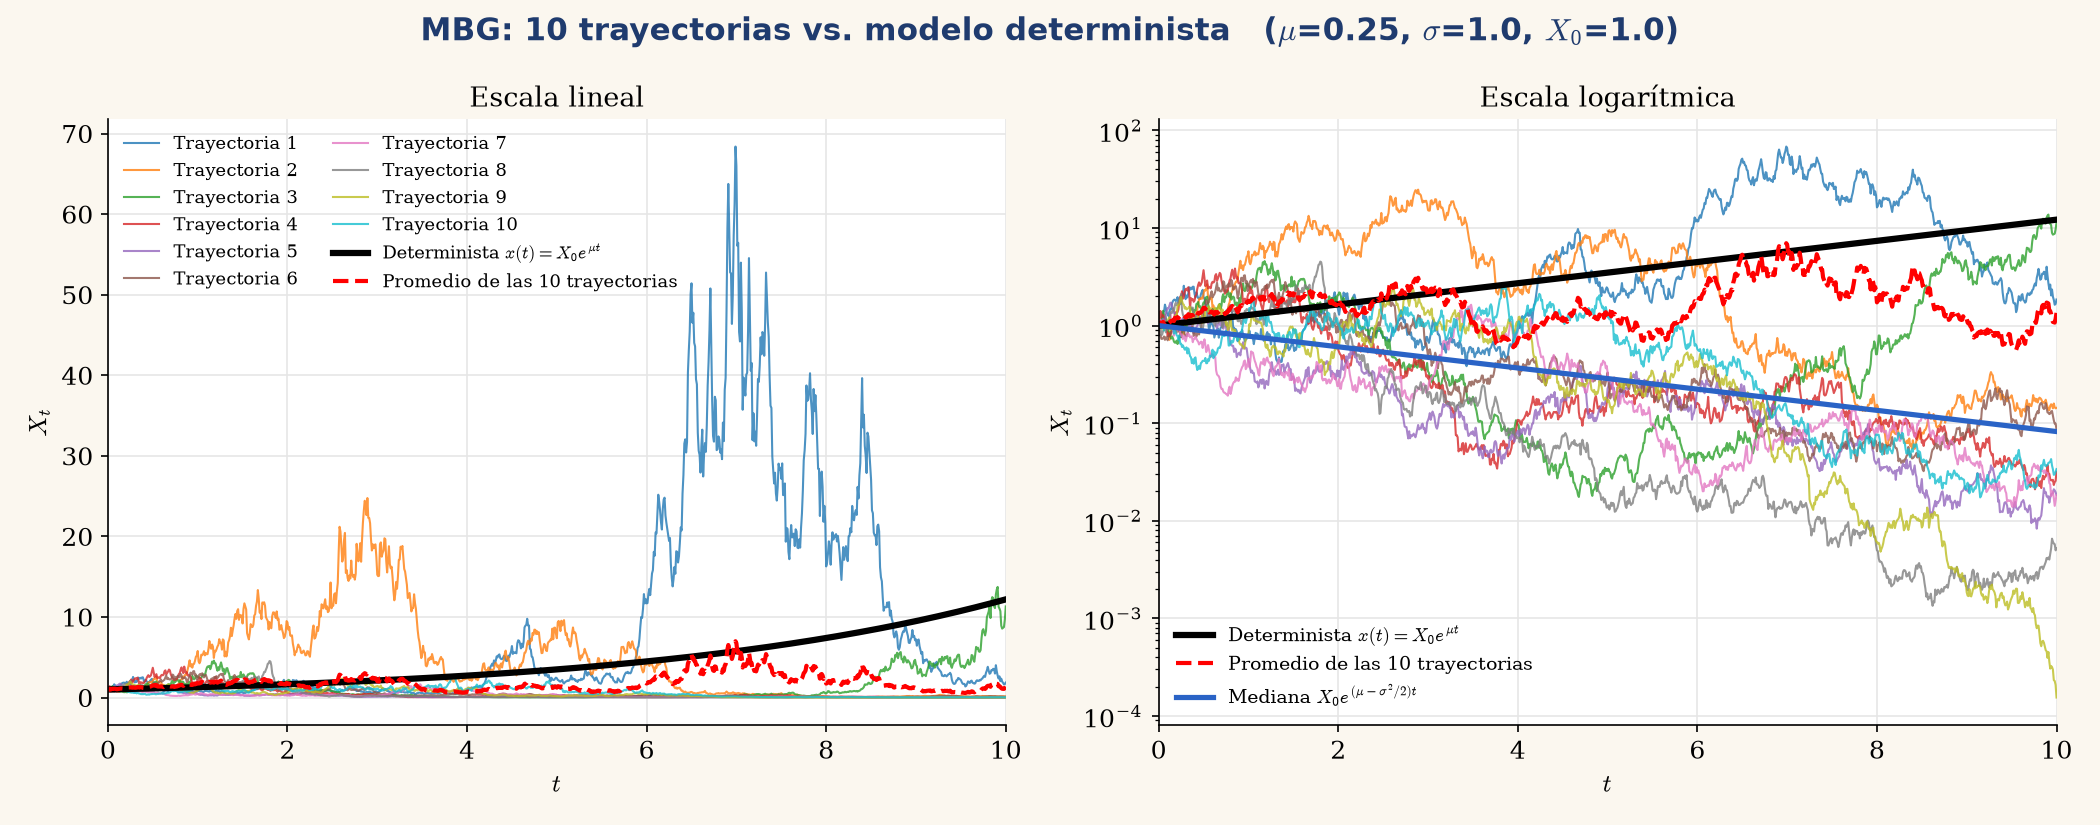
\includegraphics[width=\linewidth]{figuras_informe_mbg/resultado_mbg_vs_determinista.png}
    \caption{Diez trayectorias del MBG frente al modelo determinista $x(t) = e^{0.25t}$ (negro) y el promedio muestral (rojo discontinuo). Izquierda: escala lineal. Derecha: escala logarítmica con la mediana teórica (azul).}
    \label{fig:vsdet}
\end{figure}

Las 10 trayectorias terminan por debajo del modelo determinista, lo que es coherente con la probabilidad teórica del 94.3\,\%: la probabilidad de que las 10 queden por debajo es $0.943^{10} \approx 0.56$, así que este resultado es el más probable. El promedio ($1.3498$) está dominado por la trayectoria 3 ($X_T = 11.3090$), que por sí sola aporta $1.13$ al promedio; sin ella, el promedio de las otras nueve sería cercano a $0.24$.

Las semillas $1,\ldots,10$ son las mismas que las de las primeras 10 trayectorias del caso de la clase, así que estas 10 trayectorias son un subconjunto de las 20 de la Figura~\ref{fig:clase}.

% ============================================================
\section{Discusión}
\label{sec:discusion}
% ============================================================

\subsection{¿Por qué la media crece mientras casi todas las trayectorias decaen?}

En el caso de la clase, $\E[X_t] = e^{0.25t}$ crece, pero $\ln X_t / t \to \lambda = -0.25$, de modo que casi toda trayectoria tiende a cero. No hay contradicción: la distribución lognormal es muy asimétrica. Con $\sigma^2 T = 10$, la desviación típica teórica~\eqref{eq:varianza} en $t = 10$ es $\sqrt{e^{5}(e^{10} - 1)} \approx 1808$, unas 150 veces la media. La media se sostiene con trayectorias muy poco probables pero enormes, mientras que la gran mayoría termina cerca de la mediana, $0.0821$. Por eso la probabilidad de quedar por debajo de la media es 94.3\,\% y en la simulación las 10 trayectorias quedaron por debajo.

Interpretación práctica: el modelo determinista $\dot x = \mu x$ describe correctamente el \emph{promedio sobre muchas realizaciones}, pero no lo que le ocurre a una realización típica. Si $X_t$ representa una población o un capital, lo que ``vive'' cada sistema individual es la mediana, no la media.

\subsection{¿Por qué la media muestral se aleja de la teórica?}

La media muestral $\bar X_T = \frac1M \sum_k X_T^{(k)}$ es un estimador insesgado de $\E[X_T]$, pero su error relativo es
\begin{equation}
    \frac{\sqrt{\Var[\bar X_T]}}{\E[X_T]} = \sqrt{\frac{e^{\sigma^2 T} - 1}{M}}.
\end{equation}
Con $\sigma^2T = 10$ esto vale aproximadamente $33$ para $M = 20$ y $47$ para $M = 10$: un error del orden de miles por ciento. Para que el error relativo fuera del orden de 1 se necesitarían $M \approx e^{10} \approx 22\,000$ trayectorias. Con pocas trayectorias casi nunca aparece una de las raras trayectorias gigantes que sostienen la media, por lo que la media muestral \emph{subestima} típicamente la teórica (0.8444 y 1.3498 frente a 12.1825), y cuando por azar aparece una, la sobrestima mucho. La mediana, en cambio, depende del centro de la distribución y es mucho más estable (0.0515 frente a 0.0821).

Esta discrepancia no es un error de Euler-Maruyama: con $\Delta t = 0.01$, el sesgo débil del esquema en la media es $X_0e^{\mu T} - X_0(1 + \mu\Delta t)^N \approx 12.1825 - 12.1445 = 0.04$, despreciable frente al error de muestreo. Reducir $\Delta t$ no acerca la media muestral a la teórica; aumentar $M$ sí.

\subsection{\texorpdfstring{¿Qué pasa si $\sigma^2 < 2\mu$?}{¿Qué pasa si sigma² < 2 mu?}}

Si $\sigma^2 < 2\mu$ entonces $\lambda > 0$ y la mediana también crece: casi todas las trayectorias crecen, aunque más despacio que la media. Para comprobarlo se ejecutó \texttt{simulacion\_mbg\_clase.py --sigma 0.5}, con los demás parámetros por defecto ($\sigma^2 = 0.25 < 2\mu = 0.5$).

\begin{table}[H]
    \centering
    \caption{Salida de \texttt{simulacion\_mbg\_clase.py --sigma 0.5} en $t = T = 10$ ($M = 20$).}
    \label{tab:sigma05}
    \begin{tabular}{lrr}
        \toprule
        Estadístico & Teórico & Muestral \\
        \midrule
        $\mu - \sigma^2/2$ & $0.1250$ & --- \\
        Media   & 12.1825 & 6.2118 \\
        Mediana & 3.4903  & 2.9427 \\
        \bottomrule
    \end{tabular}
\end{table}

\begin{figure}[H]
    \centering
    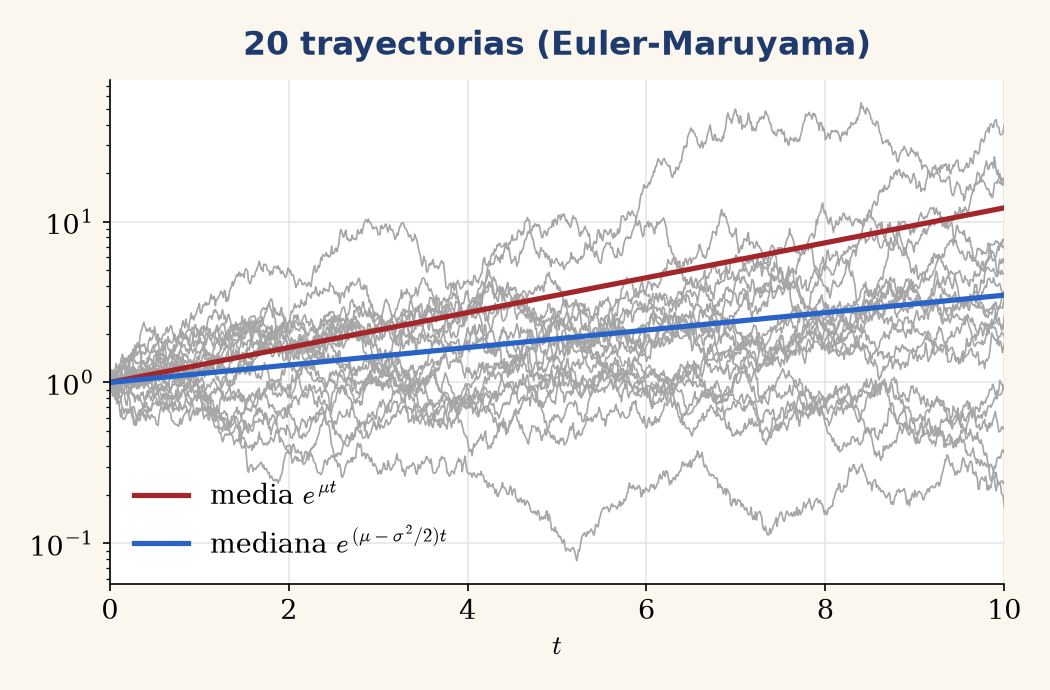
\includegraphics[width=0.85\linewidth]{figuras_informe_mbg/resultado_mbg_clase_sigma05.png}
    \caption{Veinte trayectorias con $\mu = 0.25$, $\sigma = 0.5$, $X_0 = 1$ (escala logarítmica). Ahora $\mu - \sigma^2/2 = 0.125 > 0$: la mediana crece y las trayectorias están mucho menos dispersas.}
    \label{fig:sigma05}
\end{figure}

Con menos ruido: (i) la mediana crece ($3.4903$ en $t = 10$); (ii) la media muestral ($6.2118$) se acerca mucho más a la teórica que con $\sigma = 1$, porque el error relativo esperado baja a $\sqrt{(e^{2.5} - 1)/20} \approx 0.75$; y (iii) la probabilidad de quedar por debajo del modelo determinista baja a $\Phi(0.5\sqrt{10}/2) = \Phi(0.791) \approx 0.785$ (valor calculado con la fórmula~\eqref{eq:prob}, no impreso por este script). La media sigue siendo mayor que la mediana para todo $\sigma > 0$: la brecha $e^{\sigma^2 t/2}$ crece con el ruido y con el tiempo.

% ============================================================
\section{Conclusiones}
% ============================================================

\begin{enumerate}
    \item El lema de Itô da la solución exacta del MBG, $X_t = X_0\exp[(\mu - \sigma^2/2)t + \sigma B_t]$. Su media coincide con el modelo determinista $X_0e^{\mu t}$, pero su mediana crece (o decrece) con la tasa corregida $\mu - \sigma^2/2$.
    \item El esquema de Euler-Maruyama, $X_{n+1} = X_n + \mu X_n\Delta t + \sigma X_n\sqrt{\Delta t}\,Z_n$, es la extensión natural del método de Euler; tiene orden fuerte $1/2$ y orden débil $1$.
    \item \texttt{diffeqpy} permite usar \texttt{DifferentialEquations.jl} desde Python con muy poco código: \texttt{SDEProblem} + \texttt{EM()} para la EDE y \texttt{ODEProblem} + \texttt{Tsit5()} para la EDO, con \texttt{dt}, \texttt{saveat} y \texttt{seed} para controlar el paso, la malla de salida y la reproducibilidad.
    \item Con $X_0 = 0$ la simulación estocástica coincide exactamente con la determinista (diferencia $0$), porque el ruido es multiplicativo.
    \item Con $\mu = 0.25$ y $\sigma = 1$ la media crece hasta $12.1825$ en $t = 10$, pero la mediana cae a $0.0821$; las 10 trayectorias simuladas terminaron por debajo del modelo determinista, en línea con la probabilidad teórica del 94.3\,\%.
    \item La media muestral con 10 o 20 trayectorias (1.3498 y 0.8444) no estima bien la media teórica porque la distribución lognormal tiene colas pesadas; el error se debe al muestreo, no al paso de tiempo. La mediana es un indicador mucho más estable.
    \item Si $\sigma^2 < 2\mu$, como con $\sigma = 0.5$, la mediana también crece y la media muestral se acerca a la teórica; el efecto de la corrección $-\sigma^2/2$ se vuelve menor.
\end{enumerate}

% ============================================================
\section*{Reproducibilidad}
% ============================================================

\begin{itemize}
    \item \texttt{simulacion\_mbg.py}: caso $X_0 = 0$ (EM frente a determinista). Los resultados de este informe corresponden a los parámetros del último commit ($\mu = 0.5$, $\sigma = 0.3$, $X_0 = 0$, $T = 1$, $\Delta t = 0.01$, $M = 20$).
    \item \texttt{simulacion\_mbg\_clase.py}: caso de la clase, con parámetros por línea de comandos.
    \item \texttt{simulacion\_mbg\_vs\_determinista.py}: $M$ trayectorias frente al modelo determinista.
    \item \texttt{figuras\_informe\_mbg/}: las cuatro figuras de este informe.
\end{itemize}

Para regenerar las figuras, en la carpeta del proyecto:
\begin{verbatim}
source venv/bin/activate
export PATH="$HOME/.juliaup/bin:$PATH"
export MPLBACKEND=Agg
cd figuras_informe_mbg
python3 ../simulacion_mbg.py
cd ..
python3 simulacion_mbg_clase.py \
        --salida figuras_informe_mbg/resultado_mbg_clase.png
python3 simulacion_mbg_vs_determinista.py --M 10 \
        --salida figuras_informe_mbg/resultado_mbg_vs_determinista.png
python3 simulacion_mbg_clase.py --sigma 0.5 \
        --salida figuras_informe_mbg/resultado_mbg_clase_sigma05.png
\end{verbatim}

% ============================================================
\begin{thebibliography}{9}
% ============================================================

\bibitem{higham}
D.~J. Higham, ``An algorithmic introduction to numerical simulation of stochastic differential equations'', \emph{SIAM Review}, vol.~43, n.º~3, pp.~525--546, 2001. doi:10.1137/S0036144500378302.

\bibitem{kloeden}
P.~E. Kloeden y E.~Platen, \emph{Numerical Solution of Stochastic Differential Equations}. Berlín: Springer, 1992.

\bibitem{rackauckas}
C.~Rackauckas y Q.~Nie, ``DifferentialEquations.jl -- A performant and feature-rich ecosystem for solving differential equations in Julia'', \emph{Journal of Open Research Software}, vol.~5, n.º~1, p.~15, 2017. doi:10.5334/jors.151.

\bibitem{docsde}
SciML, \emph{DifferentialEquations.jl documentation}, \url{https://docs.sciml.ai/DiffEqDocs/stable/}.

\bibitem{diffeqpy}
SciML, \emph{diffeqpy: Solving differential equations in Python using DifferentialEquations.jl}, \url{https://github.com/SciML/diffeqpy}.

\bibitem{oksendal}
B.~Øksendal, \emph{Stochastic Differential Equations: An Introduction with Applications}, 6.ª ed. Berlín: Springer, 2003.

\end{thebibliography}

\end{document}
